\documentclass[portrait,a1paper,fontscale=0.42]{baposter}

\usepackage[vlined]{algorithm2e}
\usepackage{times}
\usepackage{calc}
\usepackage{url}
\usepackage{graphicx}
\usepackage{amsmath}
\usepackage{amssymb}
\usepackage{relsize}
\usepackage{multirow}
\usepackage{booktabs}
\usepackage{mathtools}
\usepackage{multicol}
\usepackage[T1]{fontenc}
\usepackage{ae}
\usepackage{enumitem}
\usepackage{caption}
\usepackage{colortbl}
\usepackage{xcolor}
\usepackage{svg}
\svgsetup{inkscapelatex=false}
\usepackage{float}
\setlist[itemize]{leftmargin=*,nosep}
\setlength{\columnsep}{0.7em}
\setlength{\columnseprule}{0mm}

\newcommand{\compresslist}{%
\setlength{\itemsep}{0pt}%
\setlength{\parskip}{0pt}%
\setlength{\parsep}{0pt}%
}
\renewcommand{\rmdefault}{ptm}
\renewcommand{\sfdefault}{ptm}

\definecolor{hcmutblue}{RGB}{0,82,155}

%%%%%%%%%%%%%%%%%%%%%%%%%%%%%%%%%%%%%%%%%%%%%%%%%%%%%%%%%%%%%%%%%%%%%%%%%%%%%
\begin{document}
\begin{poster}{
  grid=false,
  columns=2,
  colspacing=0.8em,
  headerColorOne=hcmutblue!25!white,
  borderColor=hcmutblue!35!white,
  textborder=faded,
  headerborder=closed,
  headershape=rounded,
  headershade=plain,
  background=none,
  bgColorOne=hcmutblue!5!white,
  headerheight=0.12\textheight}
  % Eye Catcher
  {
    \includegraphics[width=0.09\linewidth]{images/Logo_BK.png}
  }
  % Title
  {\sc\huge\bf \vspace{-0.1em} Monocular 3D Object Detection for Autonomous Driving}
  % Authors
  {\vspace{0.3em}
   \textbf{Dang Vu Tuan Kiet} \\
   \vspace{0.3em}
   Supervisor: Dr.\ Nguyen Duc Dung \\
    \vspace{0.3em}
   Project code: HK252-DATN-312}
  % University logo
  {}

\begin{posterbox}[name=monodssms, column=0, row=0]{MonoDSSMs}
\begin{center}
  \includesvg[width=\linewidth]{images/monodssms/monoDSSMsOverall}
  \captionof{figure}{\small Overall architecture of MonoDSSMs.}
\end{center}

\textbf{\color{blue}Key Contributions:}
\begin{itemize}
  \item Proposed an end-to-end Mamba-based encoder-decoder architecture to extract and integrate context/depth-aware features, named Depth-Aware Mamba.
  \item The proposed architecture can achieve a comparable detection quality to the baseline, with \textbf{2.2x} fewer parameters and a \textbf{1.28x} faster computation time.
\end{itemize}

\begin{center}
  \includesvg[width=\linewidth]{images/monodssms/MambaEncoderDecoder}
  \captionof{figure}{\small (a) Mamba encoder-decoder, (b) BiMamba2, (c) CrossBiMamba2.}
\end{center}

\begin{center}
    \includesvg[width=\linewidth]{images/monodssms/BidirectionScan}
    \captionof{figure}{\small Visualization of two scanning path.}
\end{center}

\textbf{\color{blue}Results on KITTI dataset:}
\begin{center}
\small\setlength{\tabcolsep}{3pt}
\begin{tabular}{l|c|c|ccc|ccc}
  \hline
  \multirow{2}{*}{Method} & \multirow{2}{*}{FPS} & \multirow{2}{*}{Params}
    & \multicolumn{3}{c|}{Test $AP_{3D}$} & \multicolumn{3}{c}{Val $AP_{3D}$} \\
  \cline{4-9}
   & & & Easy & Mod. & Hard & Easy & Mod. & Hard \\ \hline\hline
  MonoDTR & 27.0 & 54M & 21.99 & 15.39 & 12.73 & 24.52 & 18.57 & 15.51 \\
  \hline
  MonoDSSMs-A & \textbf{34.7} & \textbf{24M} & \underline{21.47} & \underline{14.55} & 11.78 & 26.62 & 18.95 & 15.61 \\
  MonoDSSMs-M & \underline{34.5} & \textbf{24M} & 19.80 & 14.15 & 11.56 & \textbf{27.10} & \textbf{19.10} & \textbf{15.84} \\
  \hline
\end{tabular}
\end{center}

\end{posterbox}

\begin{posterbox}[name=mono3dv, column=1, row=0]%
  {Mono3DV}

\textbf{\color{blue}Motivation:}
\begin{center}
    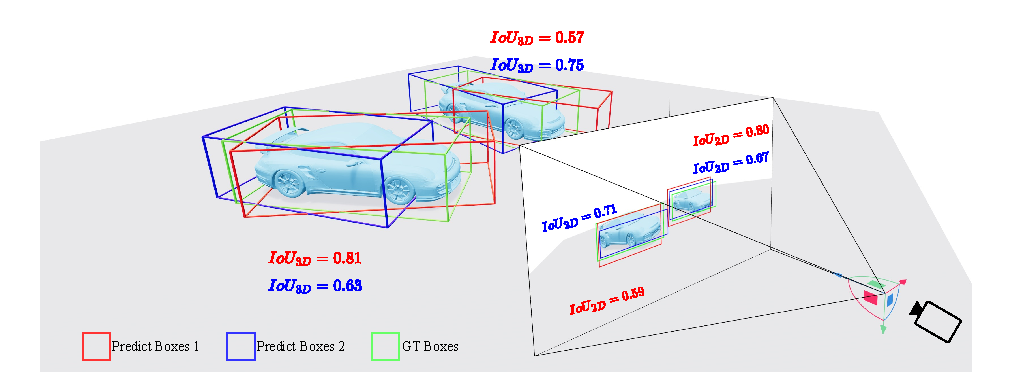
\includegraphics[width=0.95\linewidth]{images/mono3dv/motivation_3d_matching}
    \captionof{figure}{\small Problem of baseline MonoDETR.}
\end{center}

\textbf{\color{blue}Method:}
\begin{center}
  \includesvg[width=0.95\linewidth]{images/mono3dv/overall}
  \captionof{figure}{\small Overall architecture of Mono3DV.}
\end{center}

\textbf{3D-Aware Bipartite Matching} with step scheduler $\Gamma(t)$:
\[
  C_{\mathrm{match}} = C_{2D} + \Gamma(t)\,C_{3D}, \quad
  \Gamma(t) = \begin{cases} 0 & t < T \\ \epsilon & \text{otherwise} \end{cases}
\]

\textbf{Variational Query DeNoising.} VAE-based noisy query generator:

\begin{center}
  \includesvg[width=\linewidth]{images/mono3dv/motivation_vdn}
  \captionof{figure}{\small Attention entropy: VQD (VAE) vs.\ conventional denoising (AE).}
\end{center}

\textbf{\color{blue}Results on KITTI dataset:}
\begin{center}
\small\setlength{\tabcolsep}{3pt}
\begin{tabular}{l|ccc|ccc}
  \hline
  \multirow{2}{*}{Method} & \multicolumn{3}{c|}{Test $AP_{3D|R40}$}
    & \multicolumn{3}{c}{Val $AP_{3D|R40}$} \\
  \cline{2-7}
   & Easy & Mod. & Hard & Easy & Mod. & Hard \\ \hline\hline
  MonoDETR (ICCV'23) & 25.00 & 16.47 & 13.58 & 28.84 & 20.61 & 16.38 \\
  MonoCD  (CVPR'24)  & 25.53 & 16.59 & 14.53 & 26.45 & 19.37 & 16.38 \\
  MonoDGP (CVPR'25)  & \underline{26.35} & \underline{18.72} & \underline{15.97}
    & \underline{30.76} & \underline{22.34} & \underline{19.02} \\
  \hline
  \textbf{Mono3DV (Ours)} & \textbf{28.26} & \textbf{19.20} & \textbf{16.21}
    & \textbf{32.12} & \textbf{23.55} & \textbf{20.15} \\
  $\Delta$ vs.\ 2nd & \textcolor{blue}{+1.91} & \textcolor{blue}{+0.48}
    & \textcolor{blue}{+0.24} & \textcolor{blue}{+1.36} & \textcolor{blue}{+1.21}
    & \textcolor{blue}{+1.13} \\
  \hline
\end{tabular}
\end{center}

\textbf{\color{blue}Results on Waymo val set (Vehicle, Level\_1, IoU=0.7):}
\begin{center}
\small\setlength{\tabcolsep}{3pt}
\begin{tabular}{l|cccc|cccc}
  \hline
  \multirow{2}{*}{Method} & \multicolumn{4}{c|}{$AP_{3D}$} & \multicolumn{4}{c}{$APH_{3D}$} \\
  \cline{2-9}
   & All & 0--30 & 30--50 & 50--$\infty$ & All & 0--30 & 30--50 & 50--$\infty$ \\ \hline\hline
  MonoUNI   & 3.20 & 8.61 & 0.87 & 0.13 & 3.16 & 8.50 & 0.86 & 0.12 \\
  MonoDGP   & \underline{4.28} & \underline{10.24} & \underline{1.15} & \underline{0.16}
            & \underline{4.23} & \underline{10.10} & \underline{1.14} & \underline{0.16} \\
  \hline
  \textbf{Mono3DV} & \textbf{4.84} & \textbf{11.02} & \textbf{1.28} & \textbf{0.19}
                   & \textbf{4.68} & \textbf{10.78} & \textbf{1.23} & \textbf{0.18} \\
  \hline
\end{tabular}
\end{center}

\textbf{\color{blue}Plug-and-Play on nuScenes val set:}
\begin{center}
\small\setlength{\tabcolsep}{4pt}
\begin{tabular}{l|cc|ccccc}
  \hline
  Method & mAP$\uparrow$ & NDS$\uparrow$ & mATE$\downarrow$ & mASE$\downarrow$ & mAOE$\downarrow$ & mAVE$\downarrow$ & mAAE$\downarrow$ \\
  \hline
  RayDN & 46.9 & 56.3 & 0.579 & 0.264 & 0.433 & 0.256 & 0.187 \\
  \hspace{2pt}+ Ours & \textbf{47.8} & \textbf{57.1} & 0.571 & 0.262 & 0.391 & 0.273 & 0.180 \\
  \hline
  OPEN & 46.5 & 56.4 & 0.573 & 0.275 & 0.413 & 0.235 & 0.193 \\
  \hspace{2pt}+ Ours & \textbf{47.6} & \textbf{57.6} & 0.564 & 0.271 & 0.384 & 0.206 & 0.197 \\
  \hline
\end{tabular}
\end{center}

\end{posterbox}

\end{poster}
\end{document}
